\paragraph{Sơ đồ tuần tự luồng lưu trữ gói thuê bao VIP}

Luồng nghiệp vụ này mô tả
cách thức quản trị viên
(Admin)
thực hiện
lưu trữ (Archive) một gói thuê bao VIP
không còn kinh doanh
trong hệ thống để
ẩn gói thuê bao VIP
khỏi giao diện của người dùng
trong hệ thống.

\begin{figure}[H]
\centering
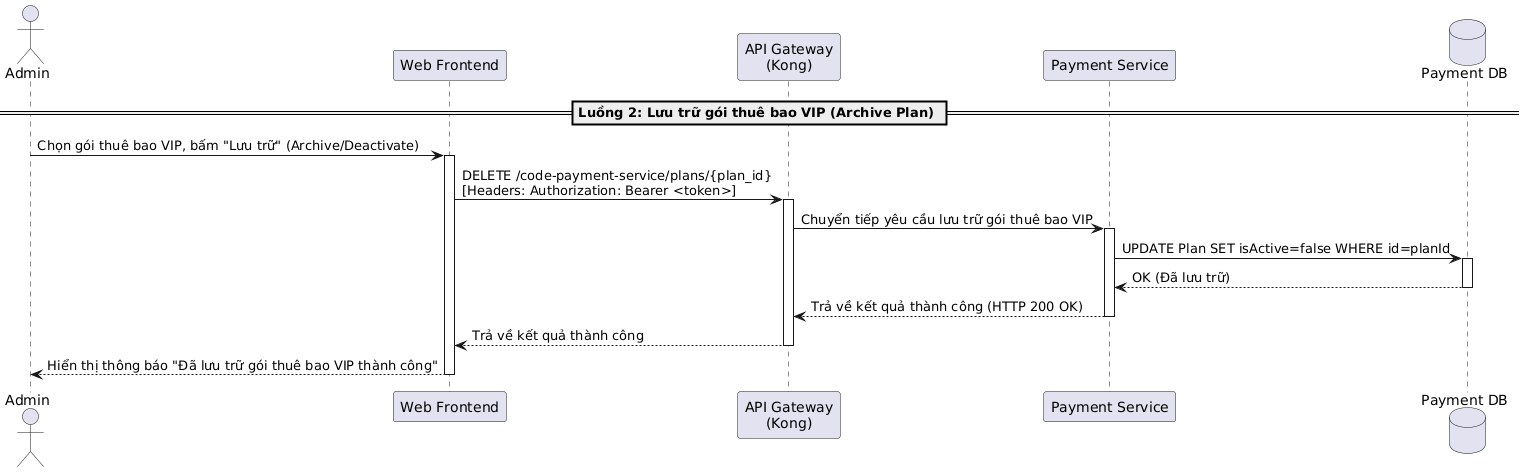
\includegraphics[width=0.95\textwidth]{contents/Sequence/UML-Sequence-AdminArchiveVipPlan.png}
\caption{Sơ đồ tuần tự luồng lưu trữ gói thuê bao VIP}
\end{figure}

\begin{table}[H]
\centering
\renewcommand{\arraystretch}{1.3}

\begin{tabular}{|l|l|p{5cm}|}
\hline
\textbf{Thành phần} & \textbf{Phân loại} & \textbf{Vai trò trong hệ thống} \\ \hline
Admin & Actor & Quản trị viên
thực hiện quản lý danh mục gói thuê bao VIP. \\ \hline
Web Frontend & Component & Giao diện web Next.js. \\ \hline
API Gateway (Kong) & Component & Cổng API chuyển tiếp các yêu cầu API. \\ \hline
Payment Service & Microservice & Tiếp nhận yêu cầu và xử lý lưu trữ các gói thuê bao VIP. \\ \hline
Payment Database & Database & Lưu trữ thông tin chi tiết về các gói thuê bao VIP (Plan). \\ \hline
\end{tabular}
\caption{Các thành phần tham gia luồng lưu trữ gói thuê bao VIP}
\end{table}

\subparagraph{Mô tả tổng quan}

\begin{itemize}
\item \textbf{Yêu cầu lưu trữ:}
Quản trị viên
tìm gói thuê bao VIP
cần dừng hoạt động
trong danh sách quản lý
và chọn tính năng lưu trữ.
\item \textbf{Gửi yêu cầu:}
Giao diện gửi yêu cầu
vô hiệu hóa gói thuê bao VIP
qua cổng API.
\item \textbf{Xử lý vô hiệu hóa:}
Dịch vụ thanh toán nhận yêu cầu,
cập nhật trạng thái gói thuê bao VIP
thành ngừng hoạt động trong CSDL
thay vì xóa hẳn để bảo toàn dữ liệu lịch sử giao dịch
và hệ thống gửi thông báo thành công về giao diện.
Gói thuê bao VIP này sẽ không còn hiển thị
và được lập lịch tự động xóa sau 30 ngày.

\end{itemize}
